\documentclass[conference]{IEEEtran}
\usepackage[utf8]{inputenc}
\usepackage[german]{babel}

\usepackage{hyperref}

\usepackage{graphicx}
\graphicspath{figures/}

\makeatletter
\let\@copyrightspace\relax
\makeatother

\begin{document}

\title{MAC Authentication Bypass (MAB)\\ in Industrie 4.0}
\author{
	Umut-Vural Mitiler\\
	u.mitiler@stud.hs-wismar.de
	\and
	Fakultät für Ingenieurwissenschaften\\
	Hochschule Wismar\\
	Master IT-Sicherheit und Forensik\\
	Industrial Security\\
	Gruppe FFM-08
	\and
	David Schunke\\
	d.schunke@stud.hs-wismar.de
}

\maketitle

\thispagestyle{plain}
\pagestyle{plain}

%

% TODO
% - durchgehen, was alles kursiv / emphasized sein soll
% - citations
% - Abstract schreiben
% - Figures austauschen, eigene draus machen, richtig referenzieren
% - Referenzen aus Handout mit reinbringen

%

\begin{abstract}
In dieser Abhandlung wird die port-based Network Access Control Methode MAC Authentication Bypass (MAB) sowie deren Bedeutung für die Industrie 4.0 diskutiert. Hierzu wird zunächst die grundsätzliche Motivation für Netzwerkzugangskontrolle dargestellt sowie eine Übersicht gegeben, was Industrie 4.0 bedeutet und definiert. Anschließend werden die technischen Grundlagen von MAB sowie den damit verbundenen Mechanismen und Standards - im speziellen Extensible Authentication Protocol (EAP) und IEEE802.1X - herausgearbeitet. Es wird zudem ein typisches Einsatzszenario als Fallback für RADIUS erläutert. Danach wird auf die Relevanz für die Industrie 4.0 sowie den bereits heute existierenden Einsatz in der Praxis eingegangen. Zum Schluss werden die Vorteile bzw. Nutzen sowie Nachteile und Gefahren diskutiert, und mögliche Gegenmaßnahmen analysiert. 
\end{abstract}

\vspace{1em}

\begin{IEEEkeywords}
MAC Authentication Bypass, MAB, EAP, Extensible Authentication Protocol, IEEE802.1X, dot1x, Network Access Control, NAC, Industrie 4.0, Schutzziele
\end{IEEEkeywords}

%

\section{Motivation}
Die fortschreitende Vernetzung von IT Systemen bahnt sich ihren weg durch alle Bereiche unseres Lebens. Während ständige Vernetzung im Privaten- sowie Dienstleistungsumfeld heute alltäglich für uns sind, ist in der Industrie ein solcher Grad an Vernetzung noch nicht angekommen. So sind häufig im industriellen Umfeld noch Maschinen oder Systeme eingesetzt, welche aufgrund ihres Alters gar keine Vernetzung und Kommunikation erlauben, als auch existierende Vernetzungen lediglich für eine einfachste Form der Kommunikation, wie z.B. Systemüberwachung, eingesetzt.\\

Industrie 4.0 stellt die aktuellste und vierte Stufe der industriellen Revolution dar. Nachdem die erste industrielle Revolution durch die Mechanisierung von Arbeitsprozessen, die zweite industrielle Revolution durch den Einsatz technischer Hilfsmittel zur Massenproduktion, und die dritte industrielle Revolution erste digitale Hilfsmittel zur Automatisierung geprägt waren, werden in der vierten industriellen Revolution alle Komponenten digitalisiert, vollumfänglich vernetzt als auch mit Intelligenz versehen, sodass diese Komponenten teils vollautonom dezentrale Entscheidungen treffen und untereinander Kommunizieren können. Der Mensch interagiert nur noch eingeschränkt und teilweise über neuartige Schnittstellen (human-computer-interfaces, HCI) mit den Systemen, um diese z.B. bei Konflikten oder benötigten Entscheidungen anzuleiten. Solche Systeme werden Cyberphysische Systeme (CPS) genannt und bilden das Rückgrat der Industrie 4.0.\\
% TODO Referenz zu den Stufen, HCI, CPS %

Mit Vernetzung und Kommunikation werden gleichzeitig solche Systeme allerdings auch stärker angreifbar und bedingen weitergehender Schutzmechanismen. Während in Office- oder User-Netzwerken
% TODO Footnote%
Technologien und Protokolle zur Absicherung der Kommunikation bereits lange zum Standard gehören, sind die in der Industrie noch häufig eingesetzten Systeme und Protokolle auf eine Absicherung noch nicht ausgelegt. Gefahren bilden hierbei u.A.

\vspace{.5em}

\renewcommand{\labelenumi}{\alph{enumi})}
\begin{enumerate}
	\item Industriespionage durch Abfangen von Kommunikation oder eindringen in Systeme (Angriff auf die Vertraulichkeit)
	\item Manipulation von Kommunikation, z.B. Steuerbefehlen (Angriff auf die Integrität)
	\item Störung der (Echtzeit-)Kommunikation bis hin zu Denial-of-Service (DoS), sodass ein System komplett ausfällt (Angriff auf die Verfügbarkeit)
	\item Übernahme (Hijacking) von Systemen und missbräuchliche Verwendung oder Erpressung
\end{enumerate}

\vspace{.5em}

Die verschiedenen Gefahren stellen für die unterschiedlichen Zweige der Industrie auch unterschiedliche Schweregrade dar, sind jedoch in der Industrie 4.0 für alle Bereiche ein hochwichtiges Thema.\\

Ein zentraler Teil zur Absicherung der Schutzziele besteht darin, wer überhaupt Zugang zu einem Netzwerk bekommt, analog zur physischen Zugangsabsicherung zu einem Gebäude oder Areal. Im Alltag findet man heute zugangsoffene Wireless LAN nur noch selten. Meistens wird zur Authentifizierung ein Passwort oder auch Pre-shared Key (PSK) benötigt. Jeder mit diesem PSK kann sich zum Netzwerk verbinden. Im Bereich des wired LAN findet man allerdings auch heute noch oft völlig unbeschränkte Netzwerke, sodass jeder mit physischem Zugang sich verbinden könnte.\\

Die PSK Methode ist simpel, hat jedoch insbesondere zwei große Nachteile:
(a) es ist keine Unterscheidung der Teilnehmer möglich, d.h. jeder Teilnehmer hat auch die gleichen Möglichkeiten im Netzwerk, eine Limitierung Einzelner oder nach Gruppen ist nicht möglich, und
(b) je größer die Anzahl an Teilnehmern im Netzwerk, desto schwieriger wird es den PSK auszutauschen und zu erneuern, sodass dies mit der Zeit ein Sicherheitsrisiko darstellen kann.\\

Zur Lösung dieses Problems wurden bereits für Enterprise Netzwerke verschiedene Strategien und Technologien entwickelt, um eine Netzwerkzugangskontrolle (Network Access Acontrol, NAC) teilnehmergenau zu realisieren, und so eine genauere Authentifizierung sowie Autorisierung auf verschiedene Ressourcen in Form von Rechtevergabe zu ermöglichen.\\

Aufgrund des Alters vieler Systeme in der Industrie können diese Technologien allerdings nicht immer einfach übertragen werden, ohne Probleme in der Kompatibilität hervorzurufen, können gleichzeitig aber auch oft nicht einfach durch neue Systeme ausgetauscht werden. Dies betrifft u.A. Netzwerkdrucker, Sensoren, Kameras, älter Server, usw.\\

Aus diesem Grund werden für solche Systeme Fallback-Lösungen benötigt, sodass diese Systeme sich gegenüber der Netzwerkzugangskontrollinstanz authentifizieren und am Netzwerk teilnehmen können. Eine solche Fallback-Lösung stellt das \emph{MAC Authentication Bypass (MAB)} dar.
% todo italic stehen lassen? was alles italic / bold? %

%

\section{Technische Grundlagen}
Zur Realisierung der Netzwerkzugangskontrolle wird eine zentrale Authentifizierungsstelle (Authentication Server) eingesetzt, sogenannte AAA-Server (Authentication, Authorization, Accounting). Jede Netzwerkkomponente (Authenticator), z.B. Router oder Switch, vergewissert sich bei ankommendem Netzwerkverkehr beim Authentication Server darüber, ob der Sender (Supplicant) authorisiert ist am Netzwerk teilzunehmen. Das \emph{Institute of Electrical and Electronics Engineers (IEEE)} hat hierfür den Standard \emph{IEEE802.1X} entwickelt, welcher wiederum die Nutzung des \emph{Extensible Authentication Protocol (EAP)} empfiehlt und somit quasi eine Verkapselung des EAP in einem Standard darstellt, weshalb im Folgenden zunächst das EAP erläutert wird.

\subsection{Extensible Authentication Protocol (EAP)}
Das EAP (RFC 3748 \cite{aboba2004extensible}) ist ein von der Internet Engineering Task Force (IETF) entwickeltes Framework zur Implementierung von Authentifizierung in Netzwerken. Es stellt Funktionen für verschiedene Authentifizierungsmethoden bereit, z.B. EAP-SIM, EAP-TTLS oder EAP-over-LAN (EAPOL). \cite{1561920} In \autoref{fig:eap} wird EAP als Abstraktionsebene dargestellt.\\

\begin{figure}[hbt]
	\centering
	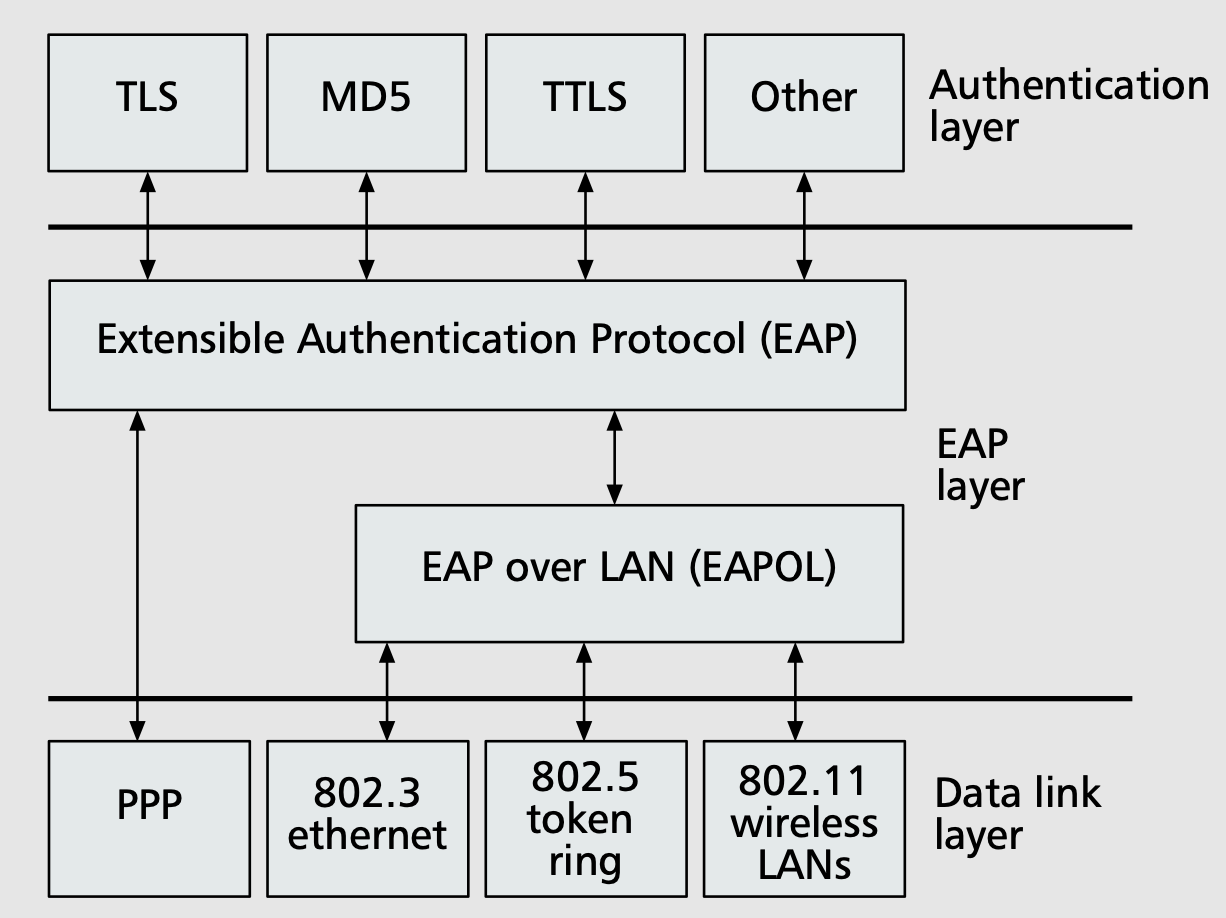
\includegraphics[width=9cm]{figures/EAP}
	\caption{EAP als Abstraktionsebene zur Authentifizierung. \cite{1561920}}
	\label{fig:eap}
\end{figure}

EAP wurde zur Unterstützung von Authentifizierung in Netzwerke geschaffen, ohne dass  bei einer neuen Authentifizierung die Infrastruktur angepasst werden müsste. Es erlaubt den Einsatz eines Authentication Servers (AAA) und implementiert die Prozesse zwischen Supplicant, Authenticator und Authentication Server. Hierbei können auch mehrere Methoden in Folge genutzt werden und erlaubt so heterogene Netzwerke. Nach Authentifizierungsanfrage (Authentication Request) vom Authenticator an den Supplicant sendet dieser eine Antwort, welche die konkrete Authentifizierung (Benutzer, Password, Zertifikat, etc.) enthält. Der Authenticator erfragt beim Authentication Server die Authentifizierung und schließt den Prozess mit einer Success- oder Failure-Response an den Supplicant ab.

\subsection{IEEE802.1X}
Der IEEE802.1X (kurz auch dot1x genannt) ist Teil der IEEE802.1 Gruppe von Standards. Es dient zur port-based Network Access Control (PNAC) und definiert Authentifizierungsmechanismen für LAN und WLAN. Hierzu setzt es auf das EAP over LAN (EAPOL) auf. In \autoref{fig:dot1x} wird die Funktionsweise und die einzelnen Parteien in dot1x dargestellt.\\

\begin{figure}[hbt]
	\centering
	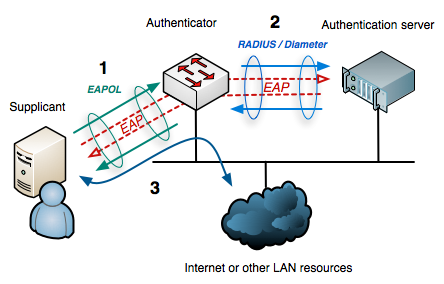
\includegraphics[width=9cm]{figures/dot1x}
	\caption{IEEE802.1X schrittweise in den einzelnen Parteien dargestellt.}
	\label{fig:dot1x}
\end{figure}

Ports werden hierbei in zwei logische Einheiten unterteilt: (1) kontrollierte Ports und (2) unkontrollierte Ports.\\
Kontrollierte Ports werden durch die dot1x PAE (Port Access Entity) gesteuert und lassen den Netzwerkverkehr für einen Supplicant entweder durch (authorized state) oder blocken diesen ab (unauthorized state).\\
Unkontrollierte Ports werden durch die dot1x PAE zur Übermittlung von EAPOL Paketen verwendet.

\subsection{RADIUS und Active Directory}
Oft als konkrete Implementierung eingesetzt werden RADIUS (Remote Authentication Dial-In User Service) oder Microsoft Active Directory. Diese bieten zentralisierte AAA-Server und sind dot1x konform, unterstützen also EAPOL. In \autoref{fig:radius} wird der Authentifizierungsprozess in Request / Response dargestellt.

\begin{figure}[hbt]
	\centering
	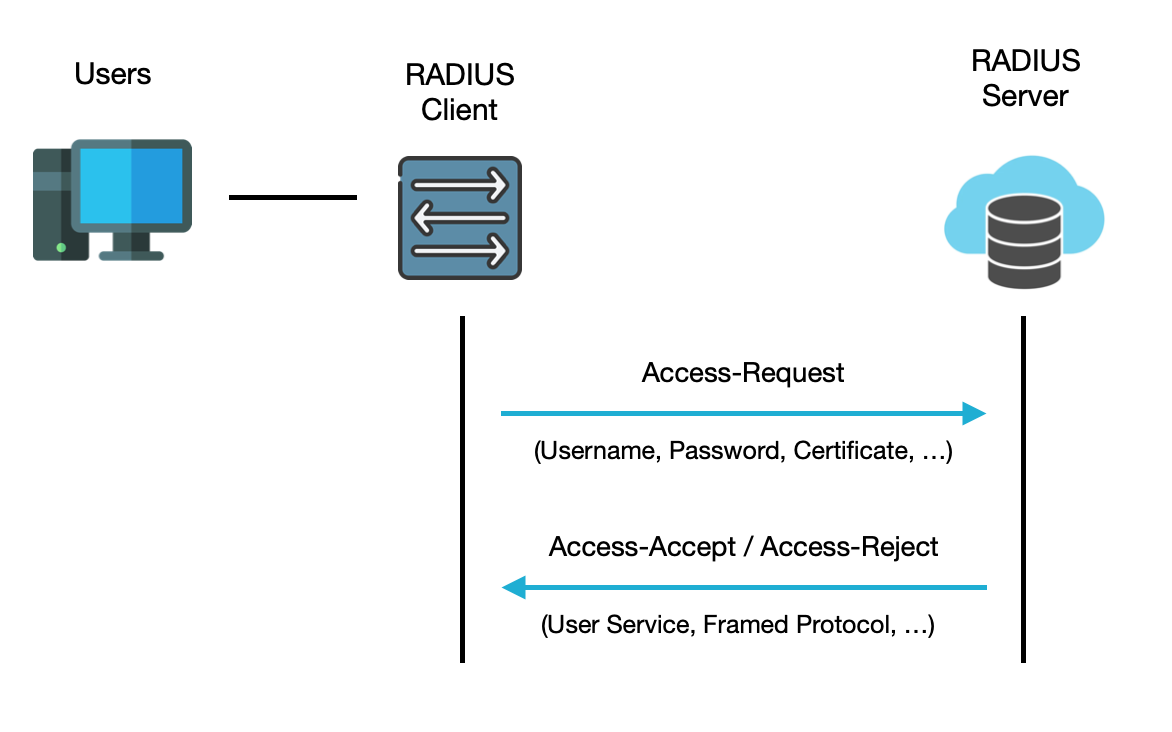
\includegraphics[width=9cm]{figures/radius}
	\caption{RADIUS Authentifizierung.}
	\label{fig:radius}
\end{figure}

\subsection{Technische Umsetzung von MAB}
MAB wird meistens als Fallback für EAP / dot1x, also z.B. RADIUS, eingesetzt. Versucht ein Supplicant sich neu zu authentifizieren wird zunächst dessen Netzwerkverkehr geblockt. Der Authenticator versucht nun den Supplicant zu authentifizieren. Hierzu wird zunächst ein EAP-Request-Identity an den Supplicant gesendet, um die Authentifizierung zu initieren. Diesen Request versteht der Supplicant allerdings nicht, da er aufgrund Alters des System oder Niedrigkosten-optimierten Herrstellung EAP nicht implementiert. Diese EAP-Requests werden wiederholt, bis ein dot1x Timeout erfolgt, woraufhin die Authentifizierung abgebrochen wird.\\

Anschließend beginnt die MAB Authentifizierung. Um die MAC-Adresse des Supplicant zu erlernen, wertet der Authenticator ein einzelnes Paket aus. Hierzu kann fast jedes beliebige Layer 2 oder 3 Paket genutzt werden. Der Authenticator sendet nun einen Access-Request an den Authentication Server. Dieser Request enthält in den Attributen \emph{Username} und \emph{Password} jeweils die MAC-Adresse des Supplicant. Lediglich das Format, in welchem die MAC-Adresse in den Attributen übertragen wird, unterscheidet sich. Zusätzlich findet sich in einigen Systemen noch das Attribute \emph{Calling-Station-ID} wieder, welches ebenfalls mit der MAC-Adresse befüllt und als sechs Gruppen mit jeweils zwei Hexadezimalstellen, in Großbuchstaben und mit Bindestrichen seperiert, übertragen wird. Welches Attribut konkret ausgewertet wird, hängt vom eingesetzten AAA-Server sowie dessen Konfiguration ab.\\

Der Authentication Server nimmt nun eine Bewertung vor und sendet entweder eine Accept oder Deny Response an den Authenticator zurück. Wichtige Voraussetzung hierzu ist, dass der Authentication Server die MAC-Adresse des Supplicant kennt, d.h. in einer Datenbank o.ä. zuvor eingepflegt wurde.\\

Der Authenticator erhält bei Erfolg ein Accept zurück und hat nun die MAC-Adresse des Supplicant erlernt. Der Supplicant ist nun auf diesem Port authentifiziert (authorised state) und kann Kommunizieren.

In \autoref{fig:mab-fallback} wird dieser Prozess noch einmal dargestellt.\\

\begin{figure}[hbt]
	\centering
	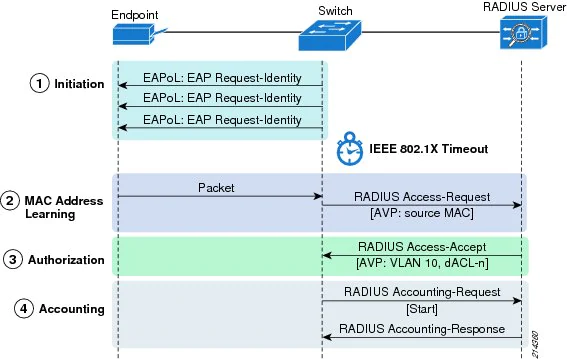
\includegraphics[width=9cm]{figures/mab-fallback}
	\caption{MAB als Fallback für RADIUS.}
	\label{fig:mab-fallback}
\end{figure}

%

\section{Praxiseinsatz}
NAC in der Praxis allgemein
\cite{mab-cisco}
\cite{mab-non-cisco}
\cite{mab-deployment-guide}

\subsection{Heutiger Einsatz}
Wie wird MAB bereits jetzt eingesetzt\\
Fallback\\
Drucker, Telefone, IP-Phones, Kameras

\subsection{Relevanz in Industrie 4.0}
Hier kommt alles zur Relevanz von Industrie 4.0\\
Skalierbarkeit, Heterogene Landschaft, Einbindung von "Leichen"

%

\section{Ergebnis}
Zusammenfassung was MAB macht, was es ist, wofür es nicht geeignet ist\\
Vorteile und Nutzen\\
Nachteile und Gefahren\\
Gegenmaßnahmen und Kombination mit anderen Technologien, wie z.B. IDS, Operational Technology, etc.\\

Wie sieht die Zukunft von MAB aus

%

\bibliographystyle{IEEEtran}
\bibliography{references}

\end{document}